%==============================================================================
\section{Desenvolvimento da Ferramenta}\label{ferramentaDeModelagemColabvorativa}
%===============================================================
Nesta seção é apresentado como foi construída a ferramenta para auxiliar na execução do processos. Na subseção \ref{ferramentaProcesso} é descrito o processo de desenvolvimento e o que foi desenvolvido. Na subseção \ref{ferramentaImplementacao} é descrito por meio de diagramas UML como está a estrutura de implementação do software.
\subsection{Processo}\label{ferramentaProcesso}
O desenvolvimento do software foi guiado por algumas atividades propostas pelo SCRUM. Como a equipe atual é constituída de dois desenvolvedores, apenas algumas atividades foram seguidas. Abaixo uma lista das atividades propostas pelo SCRUM que utilizamos.
\begin{itemize}
	\item Planejamento do Sprint
	\item Revisão do Sprint
	\item Execução do Sprint
\end{itemize}
Foi utilizado o conceito de Sprint e Sprint Backlog, no qual nos guiou em todo desenvolvimento. Definimos o tempo de cada Sprint em 2 semanas, no qual foi possível executar 2 Aprints até o desenvolvimento deste artigo. Na tabela \ref{sprintbacklog} é apresentado as histórias de usuário contidas no Sprint Backlog e na tabela \ref{sprint1} e \ref{sprint2} é apresentado as histórias de usuário executadas em cada Sprint.
\begin{table}[!htb]
	\centering
	\caption{Sprint Backlog}
		\label{sprintbacklog}
	\vspace{0.5cm}
	\begin{tabular}{r|p{11cm}|p{2cm}}
		
		ID & História de Usuário & Prioridade \\ % Note a separação de col. e a quebra de linhas
		\hline                               % para uma linha horizontal
		1 & Eu como usuário desejo poder selecionar um arquivo no formato SPEM e ter como saída uma forma de acompanhar a execução do processo.        & 1 \\
				\hline 
		2 & Eu como usuário desejo pode finalizar cada atividade do processo como intuito de acompanhar o fluxo das atividades.  & 2 \\
				\hline 
		3 & Eu como usuário desejo poder anexar arquivos nos artefatos gerados em cada uma das etapas de execução do meu processo.           & 3 \\
				\hline 
		4 & Eu como usuário desejo poder a partir de um arquivo SPEM gerar um arquivo contendo o software para execução do processo        & 4 \\         % não é preciso quebrar a última linha
		
	\end{tabular}
\end{table}

\begin{table}[!htb]

	\centering
	\caption{Sprint 1}
		\label{sprint1}
	\vspace{0.5cm}
	\begin{tabular}{r|p{11cm}|p{2cm}}
		ID & História de Usuário & Prioridade \\ % Note a separação de col. e a quebra de linhas
		\hline                               % para uma linha horizontal
		1 & Eu como usuário desejo poder selecionar um arquivo no formato SPEM e ter como saída uma forma de acompanhar a execução do processo.        & 1 
		
	\end{tabular}
\end{table}

\begin{table}[!htb]

	\centering
	\caption{Sprint 2}
		\label{sprint2}
	\vspace{0.5cm}
	\begin{tabular}{r|p{11cm}|p{2cm}}
		
		ID & História de Usuário & Prioridade \\ % Note a separação de col. e a quebra de linhas
		\hline     
		2 & Eu como usuário desejo pode finalizar cada atividade do processo como intuito de acompanhar o fluxo das atividades.  & 2 \\
		\hline 
		3 & Eu como usuário desejo poder anexar arquivos nos artefatos gerados em cada uma das etapas de execução do meu processo.           & 3 
	\end{tabular}
\end{table}

\subsection{Implementação}\label{ferramentaImplementacao}
O software foi criado utilizando a linguagem de programação JAVA com seus recursos da plataforma WEB. Abaixo é apresentado as principais tecnologias utilizadas para construção do software.
\begin{itemize}
	\item JSF
	\item Primefaces
	\item Bootstrap
	\item XStream
	\item Maven
\end{itemize}

O artigo não entrará em detalhes de implementação, apresentando apenas a relação entre as classes e a arquitetura do software.

Na subseção \ref{subsection:arquitetura} é apresentado a arquitetura do software, descrevendo o objetivo de cada pacote de software. Na subseção \ref{subsection:classes} são apresentadas as relações entre as classes do software, descrevendo de forma simplificada a funcionalidade das principais classes envolvidas na geração do diagrama de classes.

\subsubsection{Arquitetura}\label{subsection:arquitetura}
A figura \ref{figura:figuraArquitetura} apresenta os principais pacotes envolvidos na geração da estrutura para controlar a execução de processos. Os pacotes model e diagram estão envolvidos com as regras de negócio do software. Os pacotes parse e converter estão envolvidos com a conversão do modelo SPEM representado em XML para objetos no Java em tempo de execução do software.
O pacote controler tem como responsabilidade utilizar todos os demais pacotes oferecendo uma interface para o pacote view executar requisições do usuário. 
\begin{figure}[!htb]
	\caption{Arquitetura}
	\label{figura:figuraArquitetura}
	\centering
	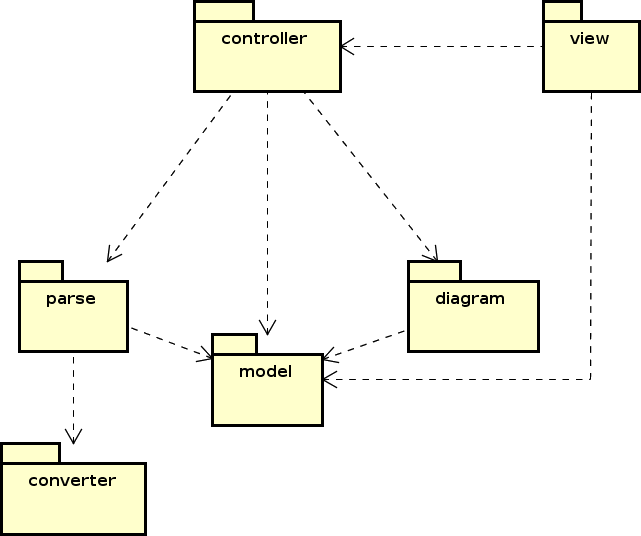
\includegraphics[width=1\textwidth]{img/ferramenta_arquitetura.png}
\end{figure}

\subsubsection{Diagrama de Classes}\label{subsection:classes}

Na figura \ref{figura:diagramaclasses} é apresentado o diagrama de classes, constituído das principais classes envolvidas na construção do software.

\begin{figure}[!htb]
	\caption{Diagrama de Classes}
	\label{figura:diagramaclasses}
	\centering
	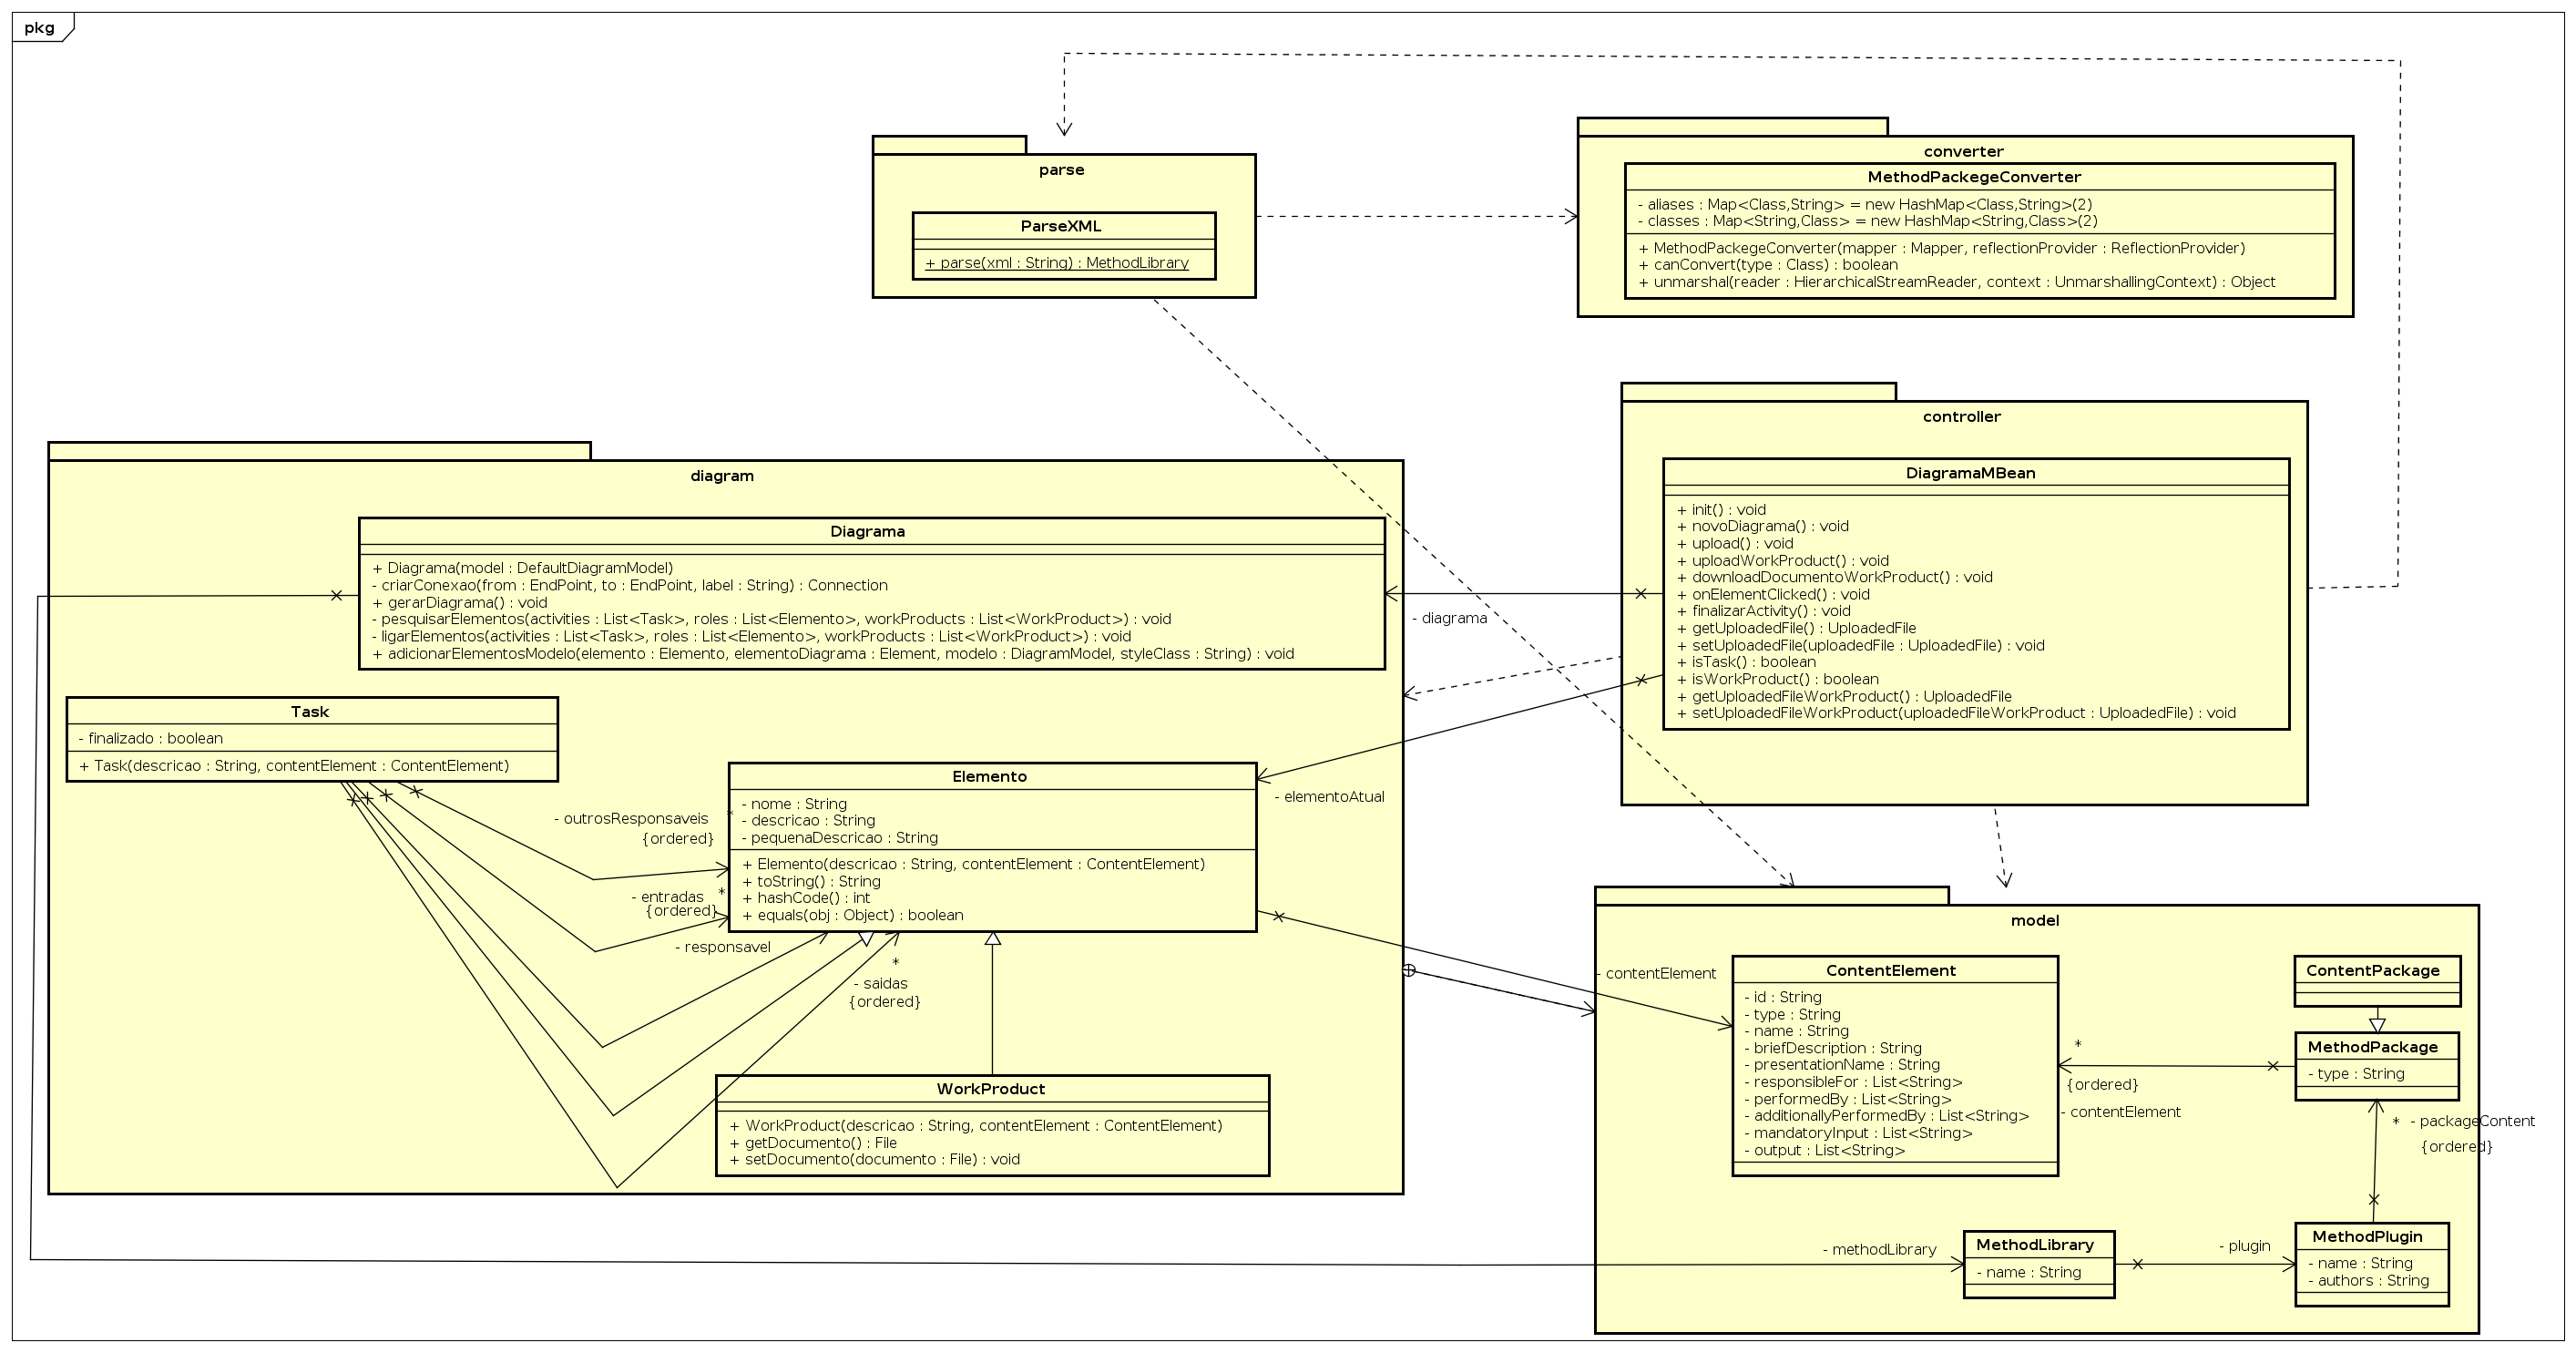
\includegraphics[width=1\textwidth]{img/ferramenta_diagrama_classes.png}
\end{figure}


